%% ============ SECTION 3 ============ %%
\newpage
\section{ Problem 3.}
\textit{
  Let $C$ be the intersection of the surface $x^2 + y^2 + z^2 = 9$ and the cylinder $x^2 + 3y^2 = 4,\quad z > 0$.
  \begin{enumerate}[label=(\alph*)]
    \item Draw the surfaces and the curve $C$.
    \item Find the length of the curve.
    \item At any given point $(x_0, y_0, z_0)$ belongs to the curve, draw the unit tangent vector.  
  \end{enumerate}
}

\vspace*{1cm}

\textbf{Theory: Finding the length of a curve using line integral.} \\
Suppose that a curve $C$ is defined by equation $y=f(x)$, where $f$ is continuous and $a \leq x \leq b$. We obtain a polygonal approximation to $C$ by dividing the interval $[a,b]$ into $n$ subintervals with endpoints $x_0,x_1,...,x_n$ and equal with $\Delta x$. If $y_i=f(x_i)$, and then the point $P_i(x,y)$ lies on $C$ and the polygon with vertices $P_0,P_1,...,P_n$, Illustrated in the below figure, is an approximation to $C$.\\[6pt]
\begin{figure}[H]
  \centering
  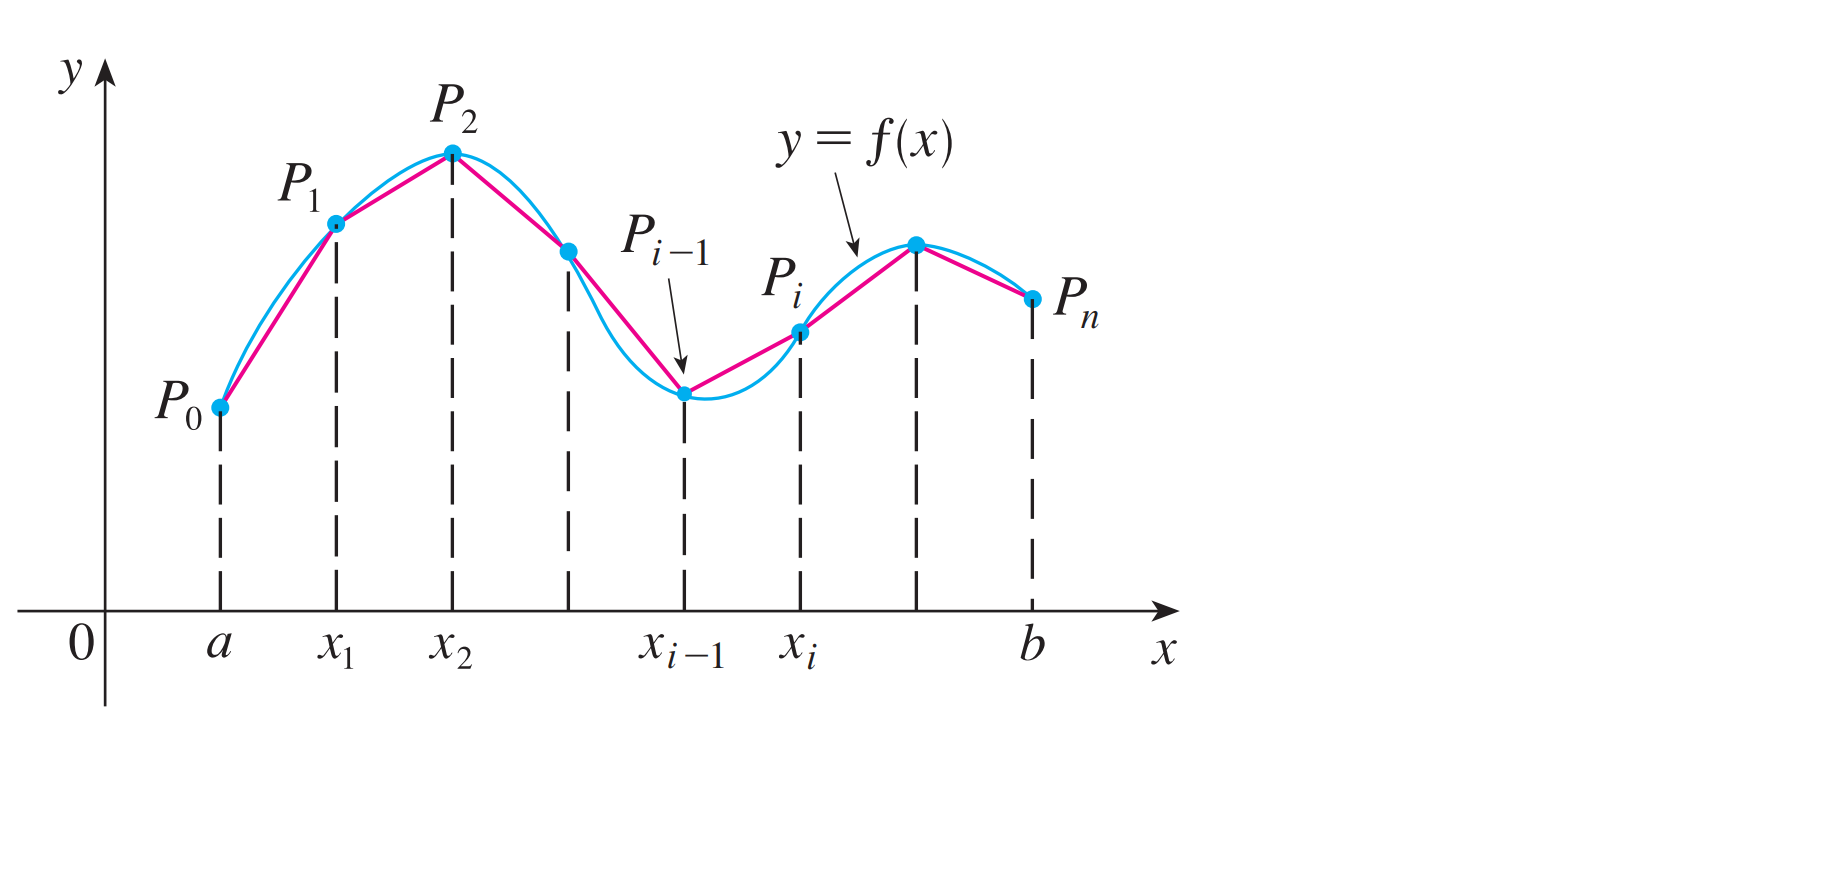
\includegraphics[width=6cm]{graphics/3_0.png}
  % \caption{}
\end{figure}
The length $L$ of is approximately the length of this polygon and the approximation gets better as we let $n$ increase. Therefore we define the length $\mathbf{L}$ of the curve $C$ with equation $y=f(x)$, $a \leq x \leq b$, as the limit of the lengths of these inscribed polygons (if the limit exists):
$$ L = \lim_{n \to \infty} \sum_{i = 1}^{n}  \left| P_{i-1} P_i \right| $$
If we let $\Delta x_i=x_i-x_{i-1}$ and $\Delta y_i=y_i-y_{i-1}$, then
$$ \left| P_{i-1} P_i \right| = \sqrt{(x_i-x_{i-1})^2 + (y_i-y_{i-1})^2} = \sqrt{(\Delta x)^2 + (\Delta y)^2} $$
By applying \textbf{the Mean Value Theorem} to $f$ on the interval $[x_{i-1},x_i]$, we find that there exist a number $x_i*$ between $x_{i-1}$ and $x_i$ such that
$$ f(x_i)-f(x_{i-1})=f(x)(x_i-x_{i-1})$$
$$ \rightarrow \Delta y_i = f'(x_i)\Delta x $$
Thus we have:
$$ \left| P_{i-1} P_i \right| = \sqrt{1^2 + [f'(x)]^2} dx $$
By the definition, this integral exists because the function $g(x) = \sqrt{1^2 + [f'(x)]^2}$ is continuous. Thus we have proved the following theorem:
If $f'$ is continuous on $[a,b]$, then the length of the curve $y=f(x)$, $a \leq x \leq b$, is
$$ L = \int_{a}^{b} \sqrt{1^2 + \left[f'(x)\right]^2} dx  $$

Then we have another assumption that $C$ can be described by the parametric equations $x=f(t)$ and $y=g(t)$, $\alpha \leq x \leq \beta$, where \vspace{0.2cm} $\dfrac{dx}{dt}=f'(t)>0$. This means that $C$ is traversed once, from left to right, as $t$ increased from $\alpha$ to $\beta$ and $f(\alpha)=a, f(\beta)=b$. We obtain:
$$ L = \int_{a}^{b} \sqrt{1^2 + \left[f'(x)\right]^2} dx = \int_{\alpha}^{\beta} \sqrt{\left(\dfrac{dx}{dt}\right)^2 + \left(\dfrac{dy}{dt}\right)^2} dx  $$

The length of space curve is defined in exactly the same way. Suppose that the curve has the vector equation $r(t)=\langle f(t), g(t), h(t) \rangle$, $a\leq x\leq b$, or, equivalently, the parametric equations $x=f(t), y=g(t), z=h(t),$ where $f',g'$ and $h'$ are continuous. If the curve is traversed exactly once as t increases from $a$ to $b$, then it can be shown that its length is
$$ L = \int_{a}^{b} \sqrt{\left[f'(x)\right]^2 + \left[g'(x)\right]^2 + \left[h'(x)\right]^2} dx = \int_{\alpha}^{\beta} \sqrt{\left(\dfrac{dx}{dt}\right)^2 + \left(\dfrac{dy}{dt}\right)^2 + \left(\dfrac{dz}{dt}\right)^2} dx  $$

\vspace*{0.5cm}

\textbf{Tangent vectors: }\\
In mathematics, a tangent vector is a vector that is tangent to a curve or surface at a given point. Tangent vectors are described in the differential geometry of curves in the context of curves in $\mathbb{R}^n$. More generally, tangent vectors are elements of a tangent space of a differentiable manifold. Tangent vectors can also be described in terms of germs. Formally, a tangent vector at the point $x$ is a linear derivation of the algebra defined by the set of germs at $x$.

Let $r(t)$ be a parametric smooth curve. The tangent vector is given by $r'(t)$ where we have used a prime instead of the usual dot to indicate differentiation with respect to parameter $t$. The unit tangent vector is given by
$$ T(x) = \dfrac{r'(x)}{\lvert r(x) \rvert} $$

\vspace*{1cm}

\textbf{MATLAB code: }\\
\textbf{\texttt{a) Draw the surfaces and the curve $C$.} }

\begin{lstlisting}[style=Matlab-editor]
  % Plot the the surface x^2 + y^2 + z^2 = 9
  f = @(x, y, z) x.^2 + y.^2 + z.^2 -9;
  fimplicit3( f , [-3 3 -3 3 0 5 ] , 'c' );  % plot the surface in cyan color
  daspect([1 1 1]) % set the aspect ratio of axes to 1 1 1
  xlabel('x');
  ylabel('y');
  zlabel('z');
  hold on;  % retain the plot for the next plot  
\end{lstlisting}

\begin{figure}[H]
  \centering
  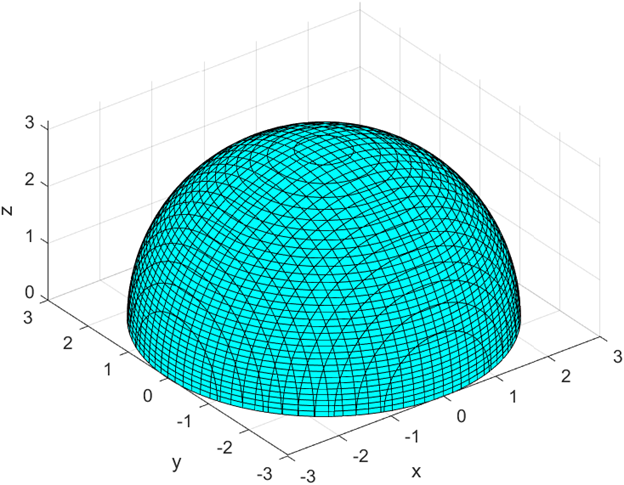
\includegraphics[width=12cm]{graphics/3a1.png}
  \caption{The surface $x^2 + y^2 + z^2 = 9$}
\end{figure}

\begin{lstlisting}[style=Matlab-editor]
% Plot the surface x^2 +3y^2 = 4
g = @(x, y) x.^2 + 3*(y.^2) -4;
fimplicit3 (g, [-3 3 -3 3 0 5 ], 'g');  % plot the surface in green color
daspect([1 1 1]) % set the aspect ratio of axes to 1 1 1
xlabel('x');
ylabel('y');
zlabel('z');
hold on;  % retain the plot for the next plot
\end{lstlisting}

\begin{figure}[H]
  \centering
  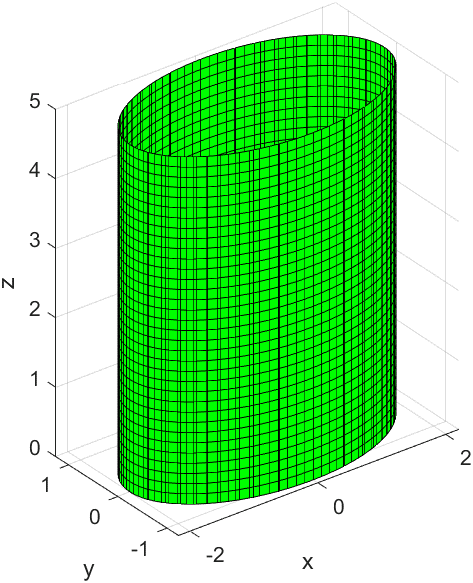
\includegraphics[width=12cm]{graphics/3a2.png}
  \caption{The cylinder $x^2 + 3y^2 = 4$}
\end{figure}

\begin{lstlisting}[style=Matlab-editor]
  % Draw the curve C as the interection of 2 surfaces:
  syms t;
  X = cos(t).*2;
  Y = sin(t).*(2/sqrt(3));
  syms t;
  X = 2.*cos(t) ;
  Y = sin(t).*(2/sqrt(3) );
  Z = sqrt(9 - 4.*cos(t).^2 - 4/3.*sin(t)^2);  % calculate the z-coordinate of the curve
  curveC = fplot3 (X, Y, Z, [ 0 2*pi ], 'linewidth', 5);
  curveC.Color = 'r';  % plot the curve with red color
  daspect([1 1 1]) % set the aspect ratio of axes to 1 1 1
  xlabel('x');
  ylabel('y');
  zlabel('z');
  title("Intersection curve of the surfaces x^2 + y^2 + z^2 = 9 and the cylinder x^2 + 3y^2 = 4, z > 0")   
\end{lstlisting}

\begin{figure}[H]
  \centering
  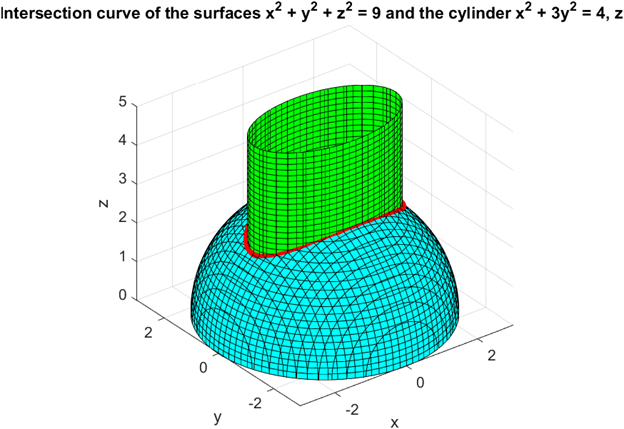
\includegraphics[width=12cm]{graphics/3a3.png}
  \caption{The surfaces and the curve $C$}
\end{figure}

\begin{lstlisting}[style=Matlab-editor]
  % Draw the curve C as the interection of 2 surfaces without line:
  syms t;
  X = cos(t).*2;
  Y = sin(t).*(2/sqrt(3));
  Z = sqrt(9 - 4.*cos(t).^2 - 4/3.*sin(t)^2);  % calculate the z-coordinate of the curve
  curveC = fplot3 (X, Y, Z, [ 0 2*pi ], 'linewidth', 3);
  curveC.Color = 'b';  % plot the curve with blue color
  daspect([1 1 1]) % set the aspect ratio of axes to 1 1 1
  xlabel('x');
  ylabel('y');
  zlabel('z');
  title("The intersection curve C of two surfaces"); 
\end{lstlisting}

\begin{figure}[H]
  \centering
  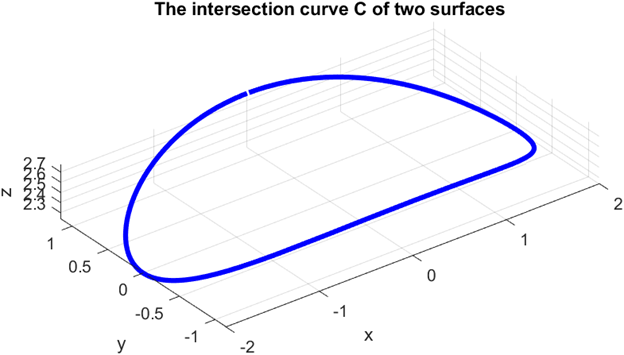
\includegraphics[width=12cm]{graphics/3a4.png}
  \caption{The intersection curve $C$}
\end{figure}

\textbf{ \texttt{b) Find the length of the curve C.} }\\

Solving by hand:\\
First we represent $x$ and $y$ through parameter $t$:
\begin{align}
  \begin{cases}
    x = 2\cos(t) \\
    y = \dfrac{2}{\sqrt{3}}\sin(t) \\
    0 \leq t \leq 2\pi\\
  \end{cases}
\end{align}
Substituing $x$ and $y$ into the equation of the cylinder $x^2 + 3y^2 = 4$, we have:
$$ z = \sqrt{  9 - 4\cos(x)^2 - \dfrac{4}{3}\sin(t)^2  } $$
Therefore the curve $C$ is defined as:
\begin{align}
  \begin{cases}
    x = 2\cos(t) \\
    y = \dfrac{2}{\sqrt{3}}\sin(t) \\
    z = \sqrt{  9 - 4\cos(x)^2 - \dfrac{4}{3}\sin(t)^2  } \\
  \end{cases}
\end{align}
The length of the curve $C$ is:
\begin{align*}
  L &= \int_{0}^{2\pi}\sqrt{\left(\dfrac{dx}{dt}\right)^2 + \left(\dfrac{dx}{dt}\right)^2 + \left(\dfrac{dx}{dt}\right)^2} dt \\
    &= \int_{0}^{2\pi}\sqrt{[-2\sin(t)]^2 + \left[\dfrac{2}{\sqrt{3}}\cos(t) \right]^2 + \left[\dfrac{8\sin(t)\cos(t)}{ 3(15+8\sin t)^2 }\right]^2} dt \\
    &= 10.3677
\end{align*}

\textbf{ \texttt{c) At any given point $(x_0, y_0, z_0)$ belongs to the curve, draw the unit tangent vector} }\\[6pt]
We have $(C)$:
\begin{align}
  \begin{cases}
    x = 2\cos(t) \\
    y = \dfrac{2}{\sqrt{3}}\sin(t) \\
    z = \sqrt{  9 - 4\cos(x)^2 - \dfrac{4}{3}\sin(t)^2  } \\
  \end{cases}
\end{align}
Let:
\begin{align*}
  r(t)  &=  2\cos(t)\hat{i} + \dfrac{2}{\sqrt{3}}\sin(t)\hat{j} + \sqrt{  9 - 4\cos(x)^2 - \dfrac{4}{3}\sin(t)^2  }    \\
  r'(t) &=  -2\sin(t)\hat{i} + \dfrac{2}{\sqrt{3}}\cos(t)\hat{j} + \dfrac{8\sin(t)\cos(t)}{ 3(15+8\sin t)^2 }     \\
\end{align*}

Therefore, we can implement this MATLAB code:
\begin{lstlisting}[style=Matlab-editor]
  % Plot the unit tangent vector at anypoint on the curve C
  t = linspace(0, 2*pi, 100);
  
  % Vector r(t)s components : x_t , y_t , z_t
  x_t = 2.*cos(t);
  y_t = 2./sqrt(3).*sin(t);
  z_t = sqrt(9 - 4.*cos(t).^2 + 4./3.*sin(t).^2);
  
  % Vector r'(t) components : m, n, p
  x = -2.*sin(t);
  y = 2./sqrt(3).*cos(t);
  z = (8.*cos(t).*sin(t))./sqrt(3.*(8.*sin(t).^2 + 15))
  
  l = sqrt(x.^2 + y.^2 + z.^2);  % length of the tangent vector
  
  m = -2*sin(t)./l;
  n = (2/sqrt(3).*cos(t))./l;
  p = (8.*cos(t).*sin(t))./sqrt(3.*(8.*sin(t).^2 + 15))./l;
  
  figure
  quiver3(x_t, y_t, z_t, m, n, p);  % plot the unit tangent vector at each point on the curve
  daspect([1 1 1]) % set the aspect ratio of axes to 1 1 1
  xlabel('x');
  ylabel('y');
  zlabel('z');
  title('Unit tangent vectors to C');
\end{lstlisting}

\begin{figure}[H]
  \centering
  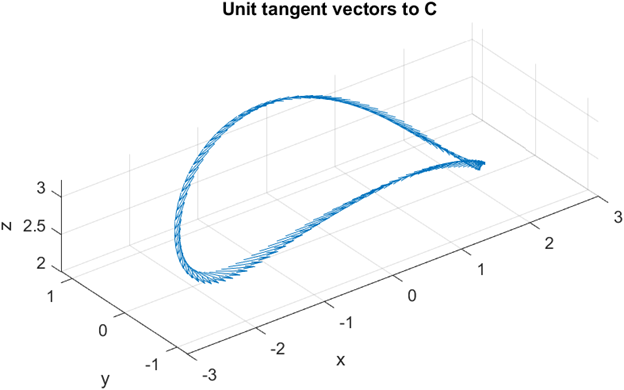
\includegraphics[width=12cm]{graphics/3c.png}
  \caption{Unit tangent vectors to $C$}
\end{figure}

\vspace*{1cm}

Code explanation:
\begin{itemize}
    \item \texttt{\color{mygreen}l = sqrt(x.$\caret$2 + y.$\caret$2 + z.$\caret$2)} - calculates the length of the unit tangent vector at each point on the curve.
    \item \texttt{\color{mygreen}m = -2*sin(t)./l} - calculates the x-component of the unit tangent vector at each point on the curve.
    \item \texttt{\color{mygreen}n = (2/sqrt(3).*cos(t))./l} - calculates the y-component of the unit tangent vector at each point on the curve.
    \item \texttt{\color{mygreen}p = (8.*cos(t).*sin(t))./sqrt(3.*(8.*sin(t).$\caret$2 + 15))./l} - calculates the z-component of the unit tangent vector at each point on the curve.
    \item \texttt{\color{mygreen}quiver3(x\_t, y\_t, z\_t, m, n, p)} - plots the unit tangent vector at each point on the curve as an arrow.
  \end{itemize}
  %\texttt{\color{mygreen}}